\section*{Results}

In order to demonstrate the efficacy of our approach, we experiment with D-NeRF's synthetic
dataset which contains 6 different scenes.

\subsection*{Quantitative Results}

Our method is able to slightly outperform D-NeRF on their synthetic dataset. This is likely because D-NeRF can predict non-realistic movement, such as jumping from frame-to-frame. In practice, D-NeRF does not do this, but the movement is not bound to have any smoothness properties, so it may not resemble real movement, by coming to full stops or suddenly accelerating. In contrast, our method enforces that movement is fluid, and thus is better able to reproduce missing frames. This only leads to a small improvement in PSNR, because the dataset contains relatively simple movement, but we expect that in longer sequences this difference would become more apparent.

\subsection*{Qualitative Results}

The difference between the architectures can be observed in the difference of flow between scenes. It's clear from Figure~\ref{fig:dnerf_cmp} that our method more accurately captures squashing and stretching of movement, as the top of the ball is not moving but the bottom of the ball is falling. In contrast, D-NeRF contains approximately equal flow for the entire ball. Since there is no forced prior on movement given by D-NeRF, there is also flow on rigid components.

The difference between the two is also more clearly seen in videos of reconstruction. $C^0$-NeRF visibly has the effect of 'tweening between views, slowing into stops, while D-NeRF has more abrupt starts and stops. While it's difficult to characterize the plausibility of this movement, future work may seek to characterize smoothness of the velocity, as well as smoothness of acceleration and use that as a way to characterize movement.

\begin{table*}[t]
    \centering
    \begin{tabular}{|c|c|c|c|c|}
    \hline
    \textbf{PSNR$^\uparrow$} & Bouncing Balls & Hellwarrior & Hook & Jumping Jacks \\
    \hline
    D-NeRF & 22.978 & 32.712 & 26.757 & 26.278 \\
    \hline
    $C^0$-NeRF & 24.251 & 33.504 & 27.705 & 27.432 \\
    \hline
    & Lego & Mutant & Standup & T-Rex \\
    \hline
    D-NeRF & 22.679 & 27.408 & 29.435 & 24.494 \\
    \hline
    $C^0$-NeRF & 22.945 & 28.486 & 31.050 & 25.421 \\
    \hline
    \end{tabular}
    \centering
    \begin{tabular}{|c|c|c|c|c|}
    \hline
    \textbf{MS-SSIM$^\uparrow$} & Bouncing Balls & Hellwarrior & Hook & Jumping Jacks \\
    \hline
    D-NeRF & 0.917 & 0.949 & 0.961 & 0.931 \\
    \hline
    $C^0$-NeRF & 0.971 & 0.966 & 0.976 & 0.978 \\
    \hline
    & Lego & Mutant & Standup & T-Rex \\
    \hline
    D-NeRF & 0.912 & 0.960 & 0.975 & 0.957  \\
    \hline
    $C^0$-NeRF & 0.935 & 0.980 & 0.988 & 0.972 \\
    \hline
    \end{tabular}
    \caption{
        Our method is able to recover movement with slightly improved accuracy in dynamic scenes as compared to D-NeRF~\cite{pumarola2020dnerf}. Despite, or maybe because of, the forced prior of continuous movement, we are able to learn a smooth interpolation through each frame. In our training regime which randomly samples all frames, we reconstruct each with much lower variance as compared to D-NeRF.
    }
\end{table*}

\begin{figure*}
    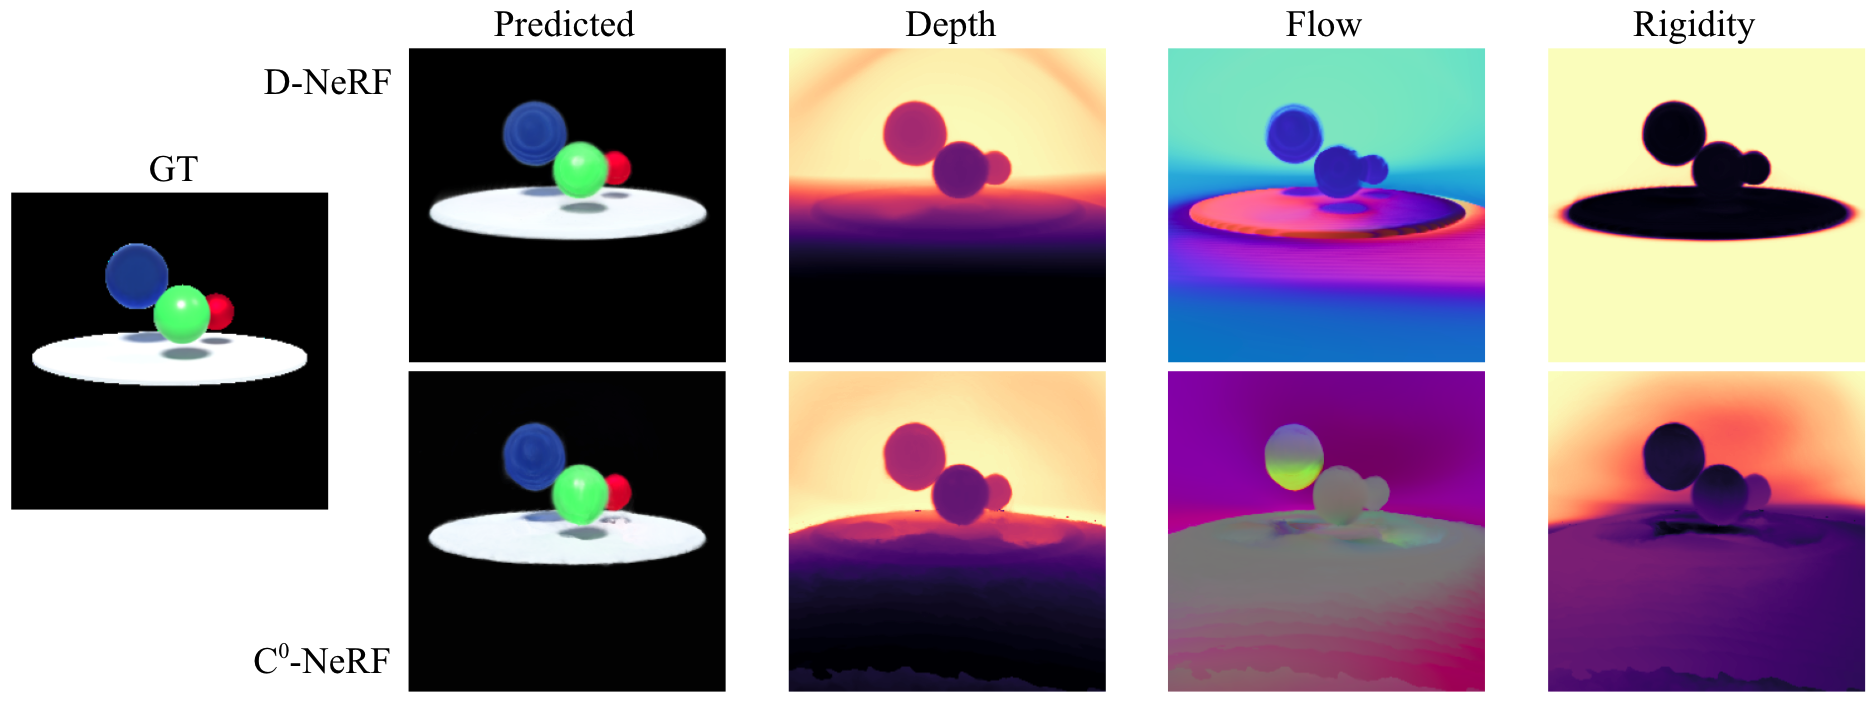
\includegraphics[width=\textwidth]{dnerf_compare}
    \caption{
        \label{fig:dnerf_cmp}
        Results comparing movement in D-NeRF~\cite{pumarola2020dnerf} versus our work for a small timestep. There is substantial qualitative difference in predicted flow, since D-NeRF cannot guarantee the initial frame has no movement. There is also a significant difference in rigidity, which is not easily explained. We assume that it may be significantly easier to model low movement with splines, thus there is less of a need for rigidity gating.
    }
\end{figure*}
